% =============================================================================
%  Team Positronic -- TEMPLATE: Sprint planning presentation (Monday, sprint start)
%  Fill every [FIELD]; keep the structure and the style.  |  SEA:ME 2.0
%  STYLE: BRUTALIST / AVANT-GARDE / INDUSTRIAL  (same as 07_presentations/sprint_00/review/present.tex)
% =============================================================================
\documentclass[11pt,aspectratio=169]{beamer}

% ----------------------------- encoding & fonts -----------------------------
\usepackage[utf8]{inputenc}
\usepackage[T1]{fontenc}
\usepackage[english]{babel}
\usepackage{helvet}
\renewcommand{\familydefault}{\sfdefault} % Sans-serif brutalista

% --------------------------------- graphics ---------------------------------
\usepackage{graphicx}
\usepackage{booktabs}
\usepackage{tabularx}
\usepackage{xcolor}
\usepackage{tikz}
\usetikzlibrary{positioning, calc, shapes.geometric, backgrounds}

\usepackage{listings}
\lstdefinestyle{pst}{
  backgroundcolor=\color{PWhite},
  basicstyle=\ttfamily\fontsize{7.5}{9}\selectfont\color{PBlack},
  keywordstyle=\color{PRed}\bfseries,
  commentstyle=\color{PGray}\itshape,
  stringstyle=\color{POrange},
  numbers=none, numberstyle=\tiny\color{PGray}, numbersep=6pt,
  showstringspaces=fadocs/07_presentations/README.mdlse, breaklines=true, breakatwhitespace=false, columns=fullflexible,
  keepspaces=true, frame=none, framerule=0pt, rulesep=0pt, rulecolor=\color{PWhite},
  xleftmargin=0pt, xrightmargin=0pt, framexleftmargin=0pt, framexrightmargin=0pt,
  aboveskip=0pt, belowskip=0pt, linewidth=\linewidth
}
\lstset{style=pst}

% ============================ BRUTAL PALETTE ============================
\definecolor{POrange}{HTML}{E86A10} % Laranja exato do logo
\definecolor{PRed}   {HTML}{D93829} % Vermelho exato do logo
\definecolor{PBlack} {HTML}{000000} % Preto Puro
\definecolor{PWhite} {HTML}{FFFFFF} % Branco Puro
\definecolor{PGray}  {HTML}{444444} % Cinza Industrial

% ================================= THEME ==================================
\setbeamertemplate{navigation symbols}{}
\setbeamercolor{background canvas}{bg=PBlack}
\setbeamercolor{normal text}{fg=PWhite}
\setbeamercolor{structure}{fg=POrange}
\setbeamercolor{itemize item}{fg=PRed}
\setbeamercolor{itemize subitem}{fg=POrange}
\setbeamersize{text margin left=1.2cm,text margin right=1.2cm}

% Marcadores de lista massivos
\setbeamertemplate{itemize item}{\raisebox{0.1ex}{\tikz\fill[PRed](0,0)rectangle(0.2,0.2);}}
\setbeamertemplate{itemize subitem}{\raisebox{0.1ex}{\tikz\fill[POrange](0,0)rectangle(0.15,0.15);}}

% --------------------------- brutal frametitle --------------------------
\setbeamertemplate{frametitle}{%
  \vspace{0.4cm}%
  \begin{tikzpicture}[remember picture, overlay]
    \fill[POrange] (current page.north west) ++(0,-0.3) rectangle ++(\paperwidth, -1.8);
    \fill[PBlack] (current page.north west) ++(0,-2.1) rectangle ++(\paperwidth, -0.2);
    \node[anchor=west, text=PBlack, font=\fontsize{24}{24}\selectfont\bfseries]
      at ([xshift=1.0cm, yshift=-1.2cm]current page.north west) {\MakeUppercase{\insertframetitle}};
    \node[anchor=east, text=PWhite, font=\fontsize{10}{10}\selectfont\bfseries]
      at ([xshift=\paperwidth-1cm, yshift=-1.2cm]current page.north west) {\MakeUppercase{\insertsectionhead}};
  \end{tikzpicture}
  \vspace{1.2cm}%
}

% -------------------------------- footline ---------------------------------
\setbeamertemplate{footline}{%
  \begin{tikzpicture}[remember picture,overlay]
    \fill[PRed] (current page.south west) rectangle ++(\paperwidth, 0.4);
    \node[anchor=west, text=PWhite, font=\fontsize{6}{6}\selectfont\bfseries\ttfamily]
      at ([xshift=1.0cm,yshift=0.2cm]current page.south west)
      {SYS: POSITRONIC // SPRINT [NN] PLANNING // SEA:ME 2.0 // RUNNING...};
    \node[anchor=east, text=PWhite, font=\fontsize{6}{6}\selectfont\bfseries\ttfamily]
      at ([xshift=\paperwidth-1.0cm,yshift=0.2cm]current page.south west)
      {FRM: \insertframenumber};
  \end{tikzpicture}%
}

% --------------------------- reusable fragments ----------------------------
\newcommand{\kw}[1]{\colorbox{PWhite}{\textcolor{PBlack}{\textbf{#1}}}}
\newcommand{\bigstat}[2]{%
  \begin{tikzpicture}[baseline]
    \fill[PGray] (0,0) rectangle (3.5, -1.8);
    \node[anchor=north west, text=POrange, font=\bfseries\fontsize{22}{22}\selectfont] at (0.2,-0.2) {#1};
    \node[anchor=south west, text=PWhite, font=\scriptsize\bfseries\ttfamily] at (0.2,-1.6) {\MakeUppercase{#2}};
  \end{tikzpicture}%
}

% avant-garde section divider: giant text, high contrast
\newcommand{\sectiondivider}[2]{%
  \begin{frame}[plain]
    \begin{tikzpicture}[remember picture,overlay]
      \fill[PRed] (current page.south west) rectangle (current page.north east);
      \node[anchor=north west, text=PBlack, font=\bfseries\fontsize{180}{150}\selectfont, inner sep=0]
        at ([xshift=-1cm, yshift=2cm]current page.north west) {#1};
      \node[anchor=south west, text=PWhite, font=\bfseries\fontsize{40}{45}\selectfont, text width=14cm]
        at ([xshift=1cm, yshift=1cm]current page.south west) {\MakeUppercase{#2}};
      \draw[PBlack, line width=10pt] ([yshift=4cm]current page.west) -- ([yshift=4cm]current page.east);
    \end{tikzpicture}
  \end{frame}%
}

% =============================================================================
\begin{document}

% ----------------------------- 00 · COVER ----------------------------------
\begin{frame}[plain]
  \begin{tikzpicture}[remember picture,overlay]
    \fill[PBlack] (current page.south west) rectangle (current page.north east);

    % Massive structural block
    \fill[PWhite] (current page.south west) ++(1,-1) rectangle ++(6.5, 10);

    % Logo integration
    % After copying to 07_presentations/sprint_NN/{planning,review}/ change the path to ../../../assets/brand/logo.png
    \node[anchor=west, fill=none, inner sep=8pt] at ([xshift=8.6cm, yshift=-1.8cm]current page.north west)
      {
\includegraphics[width=5.5cm]{../../assets/brand/logo.png}};

    % Huge Titles Bleeding
    \node[anchor=west, text=PBlack, font=\fontsize{34}{32}\selectfont\bfseries, align=left]
      at ([xshift=0.8cm, yshift=0cm]current page.west) {SPRINT\\{}[N]\\PLAN-\\NING};

    % Subtitle block
    \fill[POrange] ([xshift=7.5cm, yshift=1.0cm]current page.west) rectangle ++(8cm, -2.5cm);
    \node[anchor=west, text=PBlack, font=\large\bfseries, text width=7cm]
      at ([xshift=7.8cm, yshift=0cm]current page.west) {SPRINT [N]: [SPRINT GOAL IN AT MOST SIX WORDS]};

    % The Team
    \node[anchor=south east, text=PWhite, font=\scriptsize\bfseries\ttfamily, align=right]
      at ([xshift=-0.5cm, yshift=0.8cm]current page.south east) {
      {[FELIPE SUASSUNA]}\\
      {[LEANDRO GERTRUDES]}\\
      {[PEDRO NEIVA]}\\
      {[RUI MOURA]}\\
      {[VINÍCIUS POLATTO]}\\
      {[WALLACE LUCAS]}
    };

    % Massive Milestone Number
    \node[anchor=south west, text=PRed, font=\bfseries\fontsize{100}{100}\selectfont, inner sep=0]
      at ([xshift=7.5cm, yshift=-3.5cm]current page.west) {S[N]};
  \end{tikzpicture}
\end{frame}

% ----------------------------- 01 · ABSTRACT -------------------------------
\section*{Abstract}
\begin{frame}[plain]
  \begin{tikzpicture}[remember picture,overlay]
    \fill[POrange] (current page.south west) rectangle (current page.north east);
    \node[anchor=west, text=PBlack, font=\bfseries\fontsize{60}{60}\selectfont, rotate=90]
      at ([xshift=1.5cm, yshift=0cm]current page.west) {ABSTRACT};

    \node[anchor=north west, text=PBlack, text width=11.5cm, align=left, font=\Large\bfseries]
      at ([xshift=3.5cm, yshift=-0.2cm]current page.north west) {%
        Planning of \kw{Sprint [N]} ([MODULE]): [MON DD MMM] to [FRI DD MMM YYYY].
        \vspace{0.4cm}\\
        Goal: [one measurable sentence].%
      };
  \end{tikzpicture}
\end{frame}

% ----------------------------- 02 · AGENDA ---------------------------------
\section*{Contents}
\begin{frame}{System Index}
  \begin{columns}[T]
    \begin{column}{0.5\textwidth}
      {\large\bfseries\ttfamily
      \textcolor{PRed}{[01]} SPRINT GOAL\\
      \vspace{0.4cm}
      \textcolor{PRed}{[02]} GOALS\\
      \vspace{0.4cm}
      \textcolor{PRed}{[03]} BACKLOG\\
      \vspace{0.4cm}
      \textcolor{PRed}{[04]} TIMELINE\\
      \vspace{0.4cm}
      \textcolor{PRed}{[05]} TARGETS
      }
    \end{column}
    \begin{column}{0.5\textwidth}
      {\large\bfseries\ttfamily
      \textcolor{POrange}{[06]} RISKS\\
      \vspace{0.4cm}
      \textcolor{POrange}{[07]} REFERENCES\\
      \vspace{0.4cm}
      \textcolor{POrange}{[08]} CODE \& LESSONS\\
      \vspace{0.4cm}
      \textcolor{POrange}{[09]} CONCLUSION\\
      \vspace{0.4cm}
      \textcolor{POrange}{[10]} QUESTIONS
      }
    \end{column}
  \end{columns}
\end{frame}

% ============================== 01 · SPRINT GOAL ==============================
\section{Sprint Goal}
\sectiondivider{01}{Sprint Goal}

\begin{frame}{Sprint Goal}
  \begin{itemize}
    \setlength\itemsep{0.5em}
    \item \kw{GOAL} [one measurable sentence].
    \item Scrum Master: [name]. Module: [module].
    \item Start [Mon DD Mmm]; review \& retrospective [Fri DD Mmm].
  \end{itemize}
  \vspace{0.4cm}
  \centering
  \bigstat{[NN]}{GOALS}\hspace{0.6cm}
  \bigstat{10}{WORKING DAYS}\hspace{0.6cm}
  \bigstat{[DD MMM]}{REVIEW \& RETRO}
\end{frame}

% ============================== 02 · GOALS ==============================
\section{Goals}
\sectiondivider{02}{Goals}

\begin{frame}{Goals \& Done When}
  \begin{itemize}
    \setlength\itemsep{0.5em}
    \item G1 --- [goal 1: measurable outcome] ([issues]).
    \item G2 --- [goal 2: measurable outcome] ([issues]).
    \item G3 --- [goal 3: measurable outcome] ([issues]).
    \item G4 --- [goal 4: measurable outcome] ([issues]).
  \end{itemize}
\end{frame}

% ============================== 03 · BACKLOG ==============================
\section{Backlog}
\sectiondivider{03}{Backlog}

\begin{frame}{Backlog per Pair}
  \begin{itemize}
    \setlength\itemsep{0.6em}
    \item \kw{A} motion \& safety ([names]): [stories].
    \item \kw{B} planning \& simulation ([names]): [stories].
    \item \kw{C} quality \& measurement ([names]): [stories].
    \item One owner per story inside the pair.
  \end{itemize}
\end{frame}

% ============================== 04 · TIMELINE ==============================
\section{Timeline}
\sectiondivider{04}{Timeline}

\begin{frame}{Order of Work}
  \begin{itemize}
    \setlength\itemsep{0.6em}
    \item {}[First: what unblocks the rest].
    \item {}[Then].
    \item {}[Last].
    \item Daily standup 09:30, every working day.
    \item Review \& retrospective: [Fri DD Mmm YYYY], 15:00.
  \end{itemize}
\end{frame}

\begin{frame}{Sprint Timeline}
  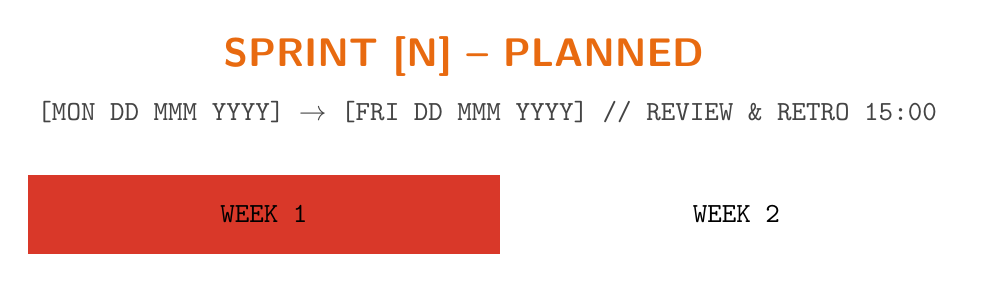
\begin{tikzpicture}
    \fill[PWhite] (0, 0) rectangle (12, 1);
    \fill[PRed] (0, 0) rectangle (6, 1);

    \node[text=PBlack, font=\bfseries\ttfamily] at (3, 0.5) {WEEK 1};
    \node[text=PBlack, font=\bfseries\ttfamily] at (9, 0.5) {WEEK 2};

    \node[anchor=west, text=PWhite, font=\Large\bfseries] at (0, 2.5) {STATUS: \textcolor{POrange}{SPRINT [N] -- PLANNED}};
    \node[anchor=west, text=PGray, font=\ttfamily] at (0, 1.8) {[MON DD MMM YYYY] $\rightarrow$ [FRI DD MMM YYYY] // REVIEW \& RETRO 15:00};
  \end{tikzpicture}
\end{frame}

% ============================== 05 · TARGETS ==============================
\section{Targets}
\sectiondivider{05}{Targets}

\begin{frame}{Targets to Measure}
  \begin{itemize}
    \setlength\itemsep{0.5em}
    \item \kw{[metric 1]} target [value + unit] --- [method].
    \item \kw{[metric 2]} target [value + unit] --- [method].
    \item \kw{[metric 3]} target [value + unit] --- [method].
    \item \kw{[metric 4]} target [value + unit] --- [method].
  \end{itemize}
\end{frame}

% ============================== 06 · RISKS ==============================
\section{Risks}
\sectiondivider{06}{Risks}

\begin{frame}{Risks}
  \begin{itemize}
    \setlength\itemsep{0.6em}
    \item {}[Risk] --- [mitigation], [owner].
    \item {}[Risk] --- [mitigation], [owner].
    \item Safety: E-stop within reach, one person moves the arm, simulation first.
  \end{itemize}
\end{frame}

% ============================== 07 · REFERENCES ==============================
\section{References}
\sectiondivider{07}{References}

\begin{frame}{References}
  \footnotesize\ttfamily
  \begin{itemize}
    \setlength\itemsep{0.5em}
    \item \textcolor{PWhite}{{[1]} [Author / project, \textit{title}, year].}
    \item \textcolor{PWhite}{{[2]} [Author / project, \textit{title}, year].}
    \item \textcolor{PWhite}{{[3]} Positronic, \textit{Sprint [N] plan} (06\_project\_management/sprints/[NN]\_sprint.md).}
  \end{itemize}
\end{frame}

% ============================== C · CODE & LESSONS ==============================
\section{Code \& Lessons}
\sectiondivider{C}{Code \& Lessons}

\begin{frame}[fragile]{Where We Start --- [TITLE]}
  
\begin{tikzpicture}
    \node[fill=PWhite, inner sep=8pt, anchor=north west] {
      \begin{minipage}{\dimexpr\textwidth-16pt\relax}
\begin{lstlisting}[frame=none, framerule=0pt, xleftmargin=0pt, xrightmargin=0pt, aboveskip=0pt, belowskip=0pt]
// [short real snippet from this sprint, at most 10 lines]
\end{lstlisting}
      \end{minipage}
    };
  \end{tikzpicture}
\end{frame}

\begin{frame}{Definition of Done}
  \begin{itemize}
    \setlength\itemsep{0.7em}
    \item PR to \texttt{dev}, \kw{TWO approvals}, \kw{CI green}.
    \item Tests added or updated, or the PR says why not.
    \item Docs updated if an interface or behaviour changed.
    \item Numbers in the PR evidence section when the story has one.
  \end{itemize}
\end{frame}

% =========================== 09 · CONCLUSION ===============================
\section{Conclusion}
\sectiondivider{09}{Conclusion}

\begin{frame}[plain]
  \begin{tikzpicture}[remember picture,overlay]
    \fill[POrange] (current page.south west) rectangle (current page.north east);

    \node[anchor=north west, text=PBlack, font=\fontsize{60}{60}\selectfont\bfseries]
      at ([xshift=1cm, yshift=-1cm]current page.north west) {CONCLUSION};

    \node[anchor=north west, text=PBlack, font=\Large\bfseries, text width=12cm]
      at ([xshift=1cm, yshift=-4cm]current page.north west) {
      [+] [NN] GOALS, ONE OWNER PER STORY.\\
      \vspace{0.4cm}
      [+] TARGETS AND METHOD FIXED.\\
      \vspace{0.4cm}
      [+] DAILY STANDUP 09:30.\\
      \vspace{0.4cm}
      [+] REVIEW \& RETRO: [FRI DD MMM].
      };
  \end{tikzpicture}
\end{frame}

% ------------------------------ 10 · Q&A -----------------------------------
\begin{frame}[plain]
  \begin{tikzpicture}[remember picture,overlay]
    \fill[PBlack] (current page.south west) rectangle (current page.north east);
    \node[anchor=center, text=PWhite, font=\bfseries\fontsize{100}{100}\selectfont]
      at (current page.center) {END\_};
    \node[anchor=south, text=POrange, font=\Large\bfseries\ttfamily]
      at ([yshift=1.5cm]current page.south) {QUESTIONS \& PLAN REVIEW};
  \end{tikzpicture}
\end{frame}

\end{document}
